%!TEX root = Main.tex

\section{Experiment}\label{Section:Experiment}

\subsection{Participants} \label{Participants}

The experiment was conducted as a Human Intelligence Task (HIT) in Amazon's Mechanical Turk \cite{crump2013evaluating, buhrmester2011amazon, stewart2015average}. There were 100 participants,  self-selected workers that saw, accepted, and finished the published HIT. We required workers to have a HIT approval rate of $95\%$ or more. Workers were informed that the payment for completing the experiment was going to be of {1.5} US dollars, 
and that 1 out of 20 participants would be randomly assigned a bonus of 10 dollars, regardless of their performance in the experiment's tasks as long as they finished the experiment (but note that trials did not end until they correctly learned each concept).

For exclusion criteria, see the appendix~\S\ref{Sec:ExclusionCriteria}.



\subsection{Experiment setup}\label{Subsec:ExperimentFlow}
The main idea of our experimental framework is schematized in Figure~\ref{fig:twoconcepts}. The participants observe an \textit{underdetermined} concept. This concept is presented to the participants as a set of elements that belong to it (positive examples), and a set of elements that do not (negative examples). In  Figure~\ref{fig:twoconcepts}, the elements marked as positive examples are the ones in the intersection of the two concepts and the negative examples are the ones outside of both concepts. Importantly, the listing is incomplete, in the sense that not all elements of the universe are shown. The critical insight is that, when extending the set of examples to the full universe, there is more than one possible concept that is consistent with the observed examples.  For example, in Figure~\ref{fig:twoconcepts},  the presented examples are consistent with the minimal rule of $C_1$ (i.e.\ $\varphi_1=p_1\lor p_2$) \textit{and also} with the minimal rule of $C_2$ (i.e.\ $\varphi_2=p_3\land p_4$). As we explain in the rest of this section, choosing $C_1$ and $C_2$ appropriately can be exploited to control the minimal rules that are consistent with the examples that participants observe.



\begin{figure}
\begin{center}
	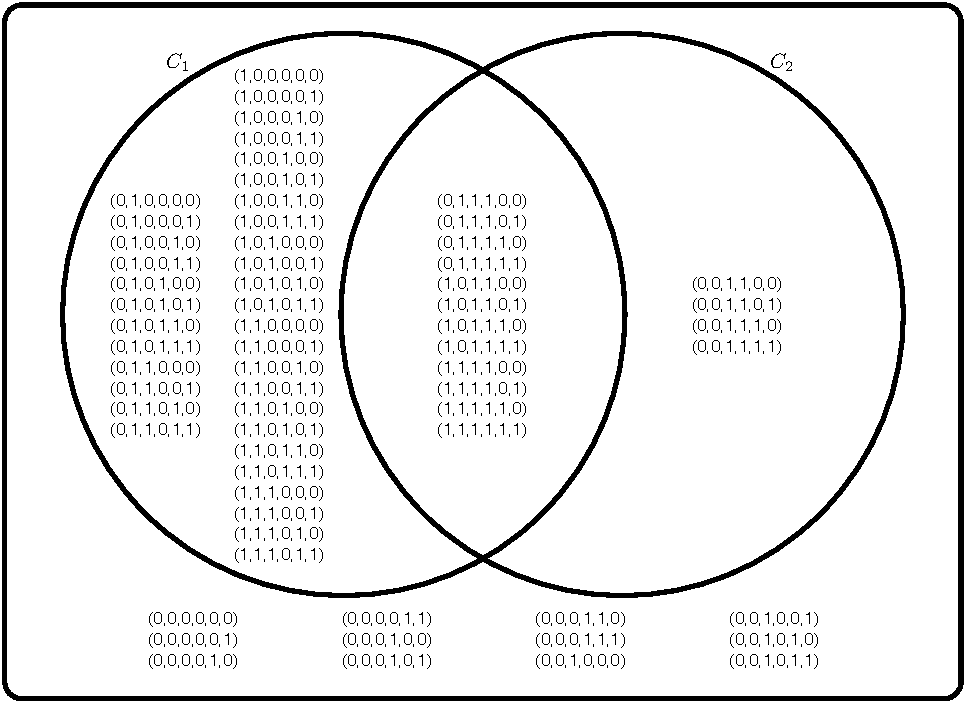
\includegraphics[scale=.65]{Images/twoconcepts3.pdf}
\end{center}\caption{An example of a pair of concepts $C_1$ and $C_2$ with 6 features. Concept $C_1$ can be described by $\varphi_1=p_1 \lor p_2$, and $C_2$ by $\varphi_2=p_3\land p_4$. This is just a schematic illustration of where each element (tuple) is placed with respect to concepts. These concepts correspond to the ones used in Trial 1 of the actual experiment. However, elements in the actual experiment are not represented in this way (i.e.\ as tuples of zeroes and ones).
}
\label{fig:twoconcepts}
\end{figure} 

The actual experiment that we implemented consists of a sequence of 6 trials constructed in this manner. We now expand the 3 stages that compose each $i$-th trial of the experiment. For a better understanding, see Figure~\ref{fig:trials}, which consists of a schematic view of one trial. Note that this figure is merely illustrative and does not aim to describe the details of a trial, but rather the sequence of phases and the logical flow within a trial. In particular, note that the number of elements {\sf A}'s, {\sf B}'s, {\sf C}'s and {\sf D}'s in the figure are not meaningful, as they vary from trial to trial along the experiment. The actual concepts used in each trial, as well as the number of positive and negative examples is listed in Table~\ref{trial_table} (groups X,Y are only relevant for Hypothesis III, so they can be ignored for now), and more details of the actual implementation can be found in \S\ref{sub:experimentdetails} and \S\ref{FullExperimentDescription}.
  
 \begin{figure}[t]
\begin{center}
	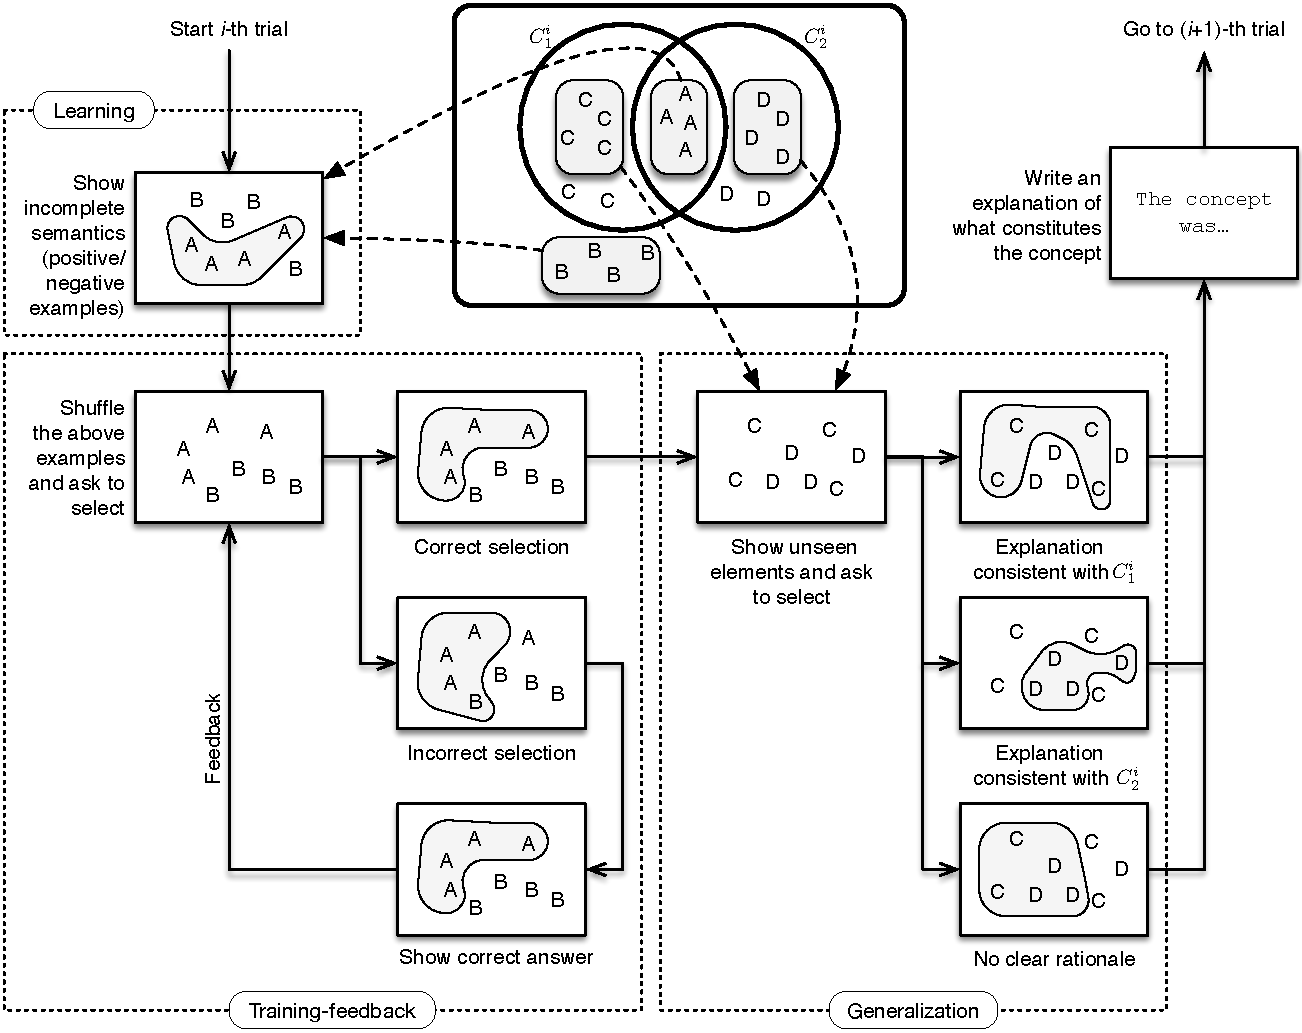
\includegraphics[scale=.7]{Images/experimentscheme2.pdf}
\end{center}\caption{The scheme of our experimental framework for studying concept learning in the presence of multiple explanations. We illustrate the three phases that constitute each trial: learning phase, training-feedback phase and generalization phase. Elements are represented with letters {\sf A}, {\sf B}, {\sf C} and {\sf D} (for example, the four letters {\sf A} in the intersection represent four different elements in the intersection). The depicted number of such letters {\sf A}, {\sf B}, {\sf C} or {\sf D} is irrelevant (for example, there would be 12 {\sf A}s and 4 {\sf D}s for concepts of Figure~\ref{fig:twoconcepts}).  }
\label{fig:trials}
\end{figure}

\begin{enumerate}
    \item \label{item:LearningStage}{\bf Learning stage.} The participant is exposed to a set of `in' elements corresponding to $C^i_1\cap C^i_2$ (marked as `{\sf A}' in Figure~\ref{fig:trials}), and a set of `out' elements corresponding to the {\em complement} of $C^i_1\cup C^i_2$ (marked as `{\sf B}' in Figure~\ref{fig:trials}). 
    
    We call these shown elements `positive examples' and `negative examples', respectively. Note that this information is incomplete, in the sense that not all possible examples are shown to the participant (as the only examples that are shown from $C^i_1\cup C^i_2$ are those in $C^i_1\cap C^i_2$). In the illustrative example of Figure~\ref{fig:twoconcepts} (corresponding to concepts of Trial 1 of the actual experiment), 24 elements would be shown: the 12 positive examples in the intersection of $C_1$ and $C_2$, and the 12 negative examples outside of both $C_1$ and $C_2$. The participant is asked to learn the concept represented by positive examples.

  As we prove formally in Appendix \ref{Sec:MainTheoremConcept}, the experimental design guarantees that there are only two propositional rules ($\varphi_1$ and $\varphi_2$ in Figure~\ref{fig:twoconcepts}), minimal over their respective sets of features, such that: \textit{(1)} they are \textit{consistent} explanations for shown examples (this is, they satisfy positive examples but do not satisfy negative examples), \textit{(2)} they use different features from each other (e.g.\ $\{p_1, p_2\}$ in $\varphi_1$ and $\{p_3,p_4\}$ in $\varphi_2$)  and, importantly, \textit{(3)} \textit{any} rule consistent with the examples must use a superset of the set of features of at least one of these minimal rules. For instance, in Figure~\ref{fig:twoconcepts} any rule that only uses $\{p_2, p_3\}$ cannot explain the examples, since $(1,{\bf 0},{\bf 1},1,1,1)$ is a positive example but  $(0,{\bf 0},{\bf 1},0,1,1)$  is a negative example. Any rule that can consistently explain the examples must mention a superset of $\{p_1, p_2\}$ (e.g.\  $\{p_1, p_2, p_3\}$) or a superset of $\{p_3, p_4\}$. The proof of this condition is shown in Theorem \ref{theorem:TeoremaPrincipal}, but we also sketch it  here. Observe that in Figure~\ref{fig:twoconcepts} the negative example  $(0,{\bf 0},{\bf 1},0,1,1)$  was constructed from the positive example  $(1,{\bf 0},{\bf 1},1,1,1)$ by flipping the values of $p_1$ and $p_4$, and doing so results in an element that is inconsistent with both $\varphi_1$ and $\varphi_2$. When an alternative explanation leaves unused some features $p,q$ that appear in $\varphi_1$ and $\varphi_2$ respectively, there must be some element that satisfies both rules $\varphi_1,\varphi_2$, but none of them is satisfied when the values of $p$ and $q$ are flipped. Since the truth value of the alternative rule is maintained when features that do not appear in it change, and since we are showing as positive examples all elements that satisfy both rules $\varphi_1,\varphi_2$ and as negative examples all those that satisfy none of them, such alternative explanation must be inconsistent with the shown data.

  These three conditions guarantee that the experimental procedure illustrated in Figure~\ref{fig:twoconcepts} is a logically sound method to present a concept consistent with two minimal rules chosen by the experimenter ($\varphi_1$ and $\varphi_2$), depending on which features the participant use to build the rule.
    

    \item {\bf Training-feedback stage.} The {\em same} examples of the learning stage are shown to the participant, but this time without indicating whether they are negative or positive and in a shuffled order. The participant is asked to tag each element as `in' or `out', in the same way they were tagged in the previous step. If all elements are classified correctly, the participant proceeds to the next stage. Otherwise, the participant is informed about the mistakes in their tagging, and after that the training-feedback stage starts again.
    
    \item {\bf Generalization stage.} {\em Previously unseen} elements are shown to the participant\footnote{With the exception of Trial 6, where one element is reshown in order to better test Hypothesis~\ref{Hip:FeatureBiasStickiness}. See \S\ref{sec:hypothesis}.}. These elements are taken from $C^i_1\setminus C^i_2$ and from $C^i_2\setminus C^i_1$ (here, `$\setminus$' denotes set difference). These elements are respectively marked as `{\sf C}' and `{\sf D}' in the scheme of Figure~\ref{fig:trials}. The participant is asked to identify those elements that correspond to the concept learnt in the learning stage. After they do so,  the next trial starts. If the participant selects those in $C^i_1\setminus C^i_2$, the concept learnt in the Learning stage was $C^i_1$, and if the participant selects those in $C^i_2\setminus C^i_1$, the concept they learned was $C^i_2$.
    Continuing with the example from Figure~\ref{fig:twoconcepts}, this process would allow us to determine if the participant was thinking in a rule with the features $\{p_1, p_2\}$ (namely, $\varphi_1$) or $\{p_3, p_4\}$ (namely, $\varphi_2$) to explain the concept. Of course, in practice the participant can select other elements, with no clear rationale.
    
    Once the participant chooses the elements, they are asked to write an explanation of what constitutes the concept; this answer is not part of the data analysis, except that it allows us to exclude participants that are using methods outside the scope of the experiment (such as taking pictures). Additionally, the written answers serve as an extra sanity check of whether the participants are actually thinking in a way consistent with the framework of propositional logic (see \S\ref{Sec:ExclusionCriteria} for observations on the written explanations obtained in the experiment).
\end{enumerate}

More details of the experiment and its structure can be found in Section~\ref{Sec:AdditionalMethodology}, particularly in \S\ref{sub:experimentdetails} and \S\ref{FullExperimentDescription}. 

\subsection{Experiment trials}\label{sec:hypothesis}
    The set of trials chosen in the experiment (Table~\ref{trial_table}) aims to reveal the biases that cause participants to choose one set of features over another in this framework where both sets of features have their own minimal rules consistent with the observed positive and negative examples. For instance, in Figure~\ref{fig:twoconcepts}, what causes participants to choose $\{p_1, p_2\}$ versus $\{p_3, p_4\}$ to explain the concept? Our hypothesis is that a key inductive bias is simply the frequency with which a subset of features was used previously to explain past concepts. We name this bias as \textit{feature stickiness}.


\renewcommand{\arraystretch}{1.4}
\newcommand{\marcaEnTabla}{{\bullet}}%\checkmark



\begin{table}[h]
\begin{center}


  \begin{tabularx}{\linewidth}{
  |>{\centering\hsize=.5\hsize}X
  |>{\centering\hsize=.7\hsize}X
  |>{\centering\hsize=.75\hsize}X
  |>{\centering\hsize=.75\hsize}X
  |>{\centering\hsize=.7\hsize}X
  |>{\centering\hsize=.3\hsize}X
  |>{\centering\hsize=.3\hsize}X
  |>{\centering\hsize=.3\hsize}X
  |>{\centering\hsize=.3\hsize}X
  |>{\centering\arraybackslash\hsize=.7\hsize}X
  |}
    \cline{1-10}
    \multirow{2}*{\textbf{Trial}}&
    \multirow{2}*{\textbf{Groups}}&
    \multirow{2}*{$\mathbf{\varphi^i_1}$}&
    \multirow{2}*{$\mathbf{\varphi^i_2}$}&
    \multirow{2}{4\baselineskip}{\textbf{\ Shown \\ features}}&
    \multicolumn{4}{c|}{\bf Tested hypotheses}&
    \multirow{2}{3\baselineskip}{\centering\tiny{\textbf{\#Positive \\ (\#Negative) \\ examples shown}}}\\
    \cline{6-9}
    &&&&&\ref{Hip:AndOverOr}&\ref{Hip:FeatureBiasStickiness}&\ref{Hip:FeatureBiasTimeAdvantage}&\ref{Hip:StickinessFeatureOperator}&\\ 
    \cline{1-10}
    $i = 1$ &  X, Y & $\varA \lor \varB$ 	& $\varC \land \varD $  & \multirow{5}*{$p_1$ to $p_6$} &$\marcaEnTabla$ & && $\marcaEnTabla$ & 12 (12) \\ \cline{1-4} \cline{6-10}
    $i = 2$&  X, Y & $\lnot \varA \land \varB$ 					& $\varC \lor \lnot \varD$ 	 &   & & &&$\marcaEnTabla$& 12 (12) \\    \cline{1-4} \cline{6-10}
    \multirow{2}*{$i = 3$} & X & $\varA \land \varB$ 	& \mdl 15   &     \multirow{2}*{} & \multirow{2}*{} &&\multirow{2}*{$\marcaEnTabla$} &&\multirow{2}*{10 (18)}\\\cline{2-4} 
     & Y & $\varE \land \varF$ 	& \mdl 15  &   &&&&&\\    \cline{1-4} \cline{6-10}
    $i = 4$&  X, Y & $ \lnot \varE \land \varF$ 					&  \mdl 15  &  &&&$\marcaEnTabla$&&10 (18)\\    \cline{1-10}
    $i = 5$&  X, Y & $\varG \land \varH$					& \mdl 15  &  \multirow{2}*{$p_3$ to $p_8$}&&$\marcaEnTabla$&&&10 (18)\\    \cline{1-4} \cline{6-10}
    $i = 6$&  X, Y & $\lnot \varG \land \lnot \varH$					& $\varC \land \varD$ &  &&$\marcaEnTabla$&&&4 (36)\\    \cline{1-10}
    \end{tabularx}

\footnotetext{In the case of $i=3$ and group A, the MDL15 rule was $((\varC \lor (\varD \lor \varE))\land(\lnot\varC \lor((\varD \lor\lnot\varE)\land(\varE \lor \lnot\varD))))$} %Uso \footnotetext porque \footnote no funciona desde la tabla
\caption{The trials of the experiment. Here $\varphi^i_1$ and $\varphi^i_2$ represent the two competing concepts $C^i_1$ and $C^i_2$ at the $i$-th trial (we denote each concept by the shortest propositional rule whose semantics describes the concept). By ``MDL15'' we denote a concept whose shortest rule is of length 15 (and made of three propositional symbols other than the competing rule in the corresponding trial, see \S\ref{Resultados:MDLbias} for details). In all trials the full universe size is $2
^6=64$, corresponding to all possible elements over 6 propositional features. We indicate how participants were divided into groups X and Y, which was used only for Hypothesis \ref{Hip:FeatureBiasTimeAdvantage}. We also indicate which features were shown in the examples, which hypothesis where tested, and the number of positive and negative examples shown in learning and training phases for each trial.}
\label{trial_table}
\end{center}
\end{table}



We now present the main hypotheses of this work, and their relation with the various experimental trials. 

\theoremstyle{definition}
\newtheorem{hyp}{Hypothesis}
\renewcommand\thehyp{\Roman{hyp}}
 

\begin{hyp}\label{Hip:AndOverOr} 
In Trial 1 we explore whether the same factors that determine rule-learning difficulty when learned in isolation also determine which features participants use when explaining a set of examples consistent with two minimal rules. Particularly, it is well known that concepts involving logical conjunctions are learned faster than concepts involving logical disjunctions \cite{bourne1970knowing}.

In Trial 1, the minimal consistent rule is a disjunction if the observed features are $\{p_1, p_2\}$, and a conjunction if the observed features are $\{p_3, p_4\}$. Importantly, unlike in other concept-learning experiments, both the two-feature disjunction and conjunction are consistent with the observed set of examples. We hypothesize that the learning bias that causes the conjunction to be learnt more easily than the disjunction will also carry over to this framework were both explanations are possible (using different features). As explained before, we use the generalization stage of Trial 1 to determine if participants understood the concept using $\{p_1, p_2\}$ (corresponding to a disjunction) or using $\{p_3, p_4\}$ (corresponding to a conjunction).


This hypothesis was preregistered as:
\begin{quote}
In a scenario of two possible explanations for a concept, one of which can be modeled by the logical \AND between two features and other which can be modeled by the \OR between two other features, most people will find the \AND explanation over the \OR explanation.% (Trial 1).     
\end{quote}
\end{hyp}

\begin{hyp}\label{Hip:FeatureBiasStickiness}

    The \textit{feature stickiness} bias is tested in Trials 5 and 6 of the experiment. After participants have gained sufficient experience with the task, in Trial 5 participants encounter a set of examples consistent with two minimal explanations, a very simple one that uses features $\{p_7, p_8\}$ and a very complex one that uses $\{p_4,p_5,p_6\}$. This leads participants to explain the concept using $\{p_7, p_8\}$, or otherwise they would have to discover an excessively complex explanation. Therefore, we hypothesize that in this case most participants would select the features $\{p_7, p_8\}$\footnote{Note that the features $\{p_5,p_6\}$ that were used in Trial 4 also appear in the MDL15 formula of Trial 5. However, we hypothesized that the extreme complexity of the MDL15 explanation overwheights the possible feature stickiness effect from Trial 4 to 5. Indeed, we found that none of the participants used the MDL15 formula in Trial 5.}. 
    
        In the following concept (Trial 6), participants must choose between explanations that use the previously useful features $\{p_7, p_8\}$, or another fresh set of features $\{p_3, p_4\}$. We hypothesize that participants are more likely to explain the concept using $\{p_7, p_8\}$, only because these features were useful in the previous concept. Also, recall that explanations that use a set of features containing either $\{p_7, p_8\}$ or $\{p_3, p_4\}$ are also compatible. For example, in Trial 6 the explanation $p_3 \land p_4 \land \lnot p_7$ is compatible with the observed examples. We are also interested in these rules (e.g.\ we think it is more likely that participants will use $\{p_7, p_8, p_3\}$ than $\{p_3, p_4, p_7\}$). The seven elements chosen for the generalization stage of Trial 6 allows us to do precisely this: 7 elements appear on the screen, with $p_3, p_4, p_7, p_8$ respectively equal to $(1, 1, 1, 1)$, $(1, 1, 0, 1)$, $(1, 1, 1, 0)$, $(1, 1, 0, 0)$, $(1, 0, 0, 0)$, $(0, 1, 0, 0)$, $(0, 0, 0, 0)$. These elements are respectively consistent with the minimal rules $p_3 \land p_4$, $p_3 \land p_4 \land \lnot p_7$, $p_3 \land p_4 \land \lnot p_7 \land \lnot p_8$, $p_3 \land \lnot p_7 \land \lnot p_8$, $p_4 \land \lnot p_7 \land \lnot p_8$ and  $\lnot p_7 \land \lnot p_8$. Importantly, none of the elements is consistent with more than one of the two minimal rules.

This hypothesis was preregistered as:
\begin{quote}
If a person has used a set of features in the construction of an explanation for a concept, it is more likely that she will also find an explanation containing those features in the following trial. 
\end{quote}
    
\end{hyp}


\begin{hyp}\label{Hip:FeatureBiasTimeAdvantage}
We address the question of whether the feature stickiness bias represents a computational advantage in itself. More concretely, we ask if participants find a consistent rule {\it faster} when they are reusing the same features as in the previous trial.  Note that this is a distinct phenomenon from Hypothesis~\ref{Hip:FeatureBiasStickiness}, which is concerned with preferential selection and not with times. 
We test this question, independently of the effect of the feature stickiness bias, in Trials 3 and 4 of the experiment. In Trial 3, we separate participants into groups X and Y. In the same manner as in Trial 5, in Trial 3 group X is biased to learn the rule using $\{p_1, p_2\}$, and group Y using $\{p_5, p_6\}$. In the next trial (Trial 4), participants are biased to learn the rule using $\{p_5, p_6\}$. We hypothesize that participants from group Y will learn concept $C^4_1$ faster than participants from group X, given that they are reusing the same features they used in the previous trial.


This hypothesis was preregistered as:
\begin{quote}
When a concept can only be reasonably described by a given set of features, a person will find this description faster if that same set of features was useful for her in the immediately previous trial.
\end{quote}
\end{hyp}

\begin{hyp} \label{Hip:StickinessFeatureOperator}


 Another question, tested with Trials 1 and 2, examines the relative strength of feature bias versus operator bias. That is, we want to determine whether there is some strong effect that clearly biases attention towards features (or rather toward operators) that have previously been found useful for describing concepts. We test this by switching the operator ($\lor$/$\land$) that each pair of features can use to form a useful rule in each trial, and by then comparing the number of participants that explain the shown examples of Trial 2 by reusing the same features from Trial 1 versus those that reused the operator but used different features.
 

 
 This hypothesis was preregistered as:
\begin{quote}
 In a scenario where both features and operators are repeated from a trial to the next, there will be a stickiness effect favoring one of them over the other.
\end{quote}

\end{hyp}